% *** Authors should verify (and, if needed, correct) their LaTeX system  ***
% *** with the testflow diagnostic prior to trusting their LaTeX platform ***
% *** with production work. IEEE's font choices can trigger bugs that do  ***
% *** not appear when using other class files.                            ***
% The testflow support page is at:
% http://www.michaelshell.org/tex/testflow/


%%*************************************************************************
%% Legal Notice:
%% This code is offered as-is without any warranty either expressed or
%% implied; without even the implied warranty of MERCHANTABILITY or
%% FITNESS FOR A PARTICULAR PURPOSE!
%% User assumes all risk.
%% In no event shall IEEE or any contributor to this code be liable for
%% any damages or losses, including, but not limited to, incidental,
%% consequential, or any other damages, resulting from the use or misuse
%% of any information contained here.
%%
%% All comments are the opinions of their respective authors and are not
%% necessarily endorsed by the IEEE.
%%
%% This work is distributed under the LaTeX Project Public License (LPPL)
%% ( http://www.latex-project.org/ ) version 1.3, and may be freely used,
%% distributed and modified. A copy of the LPPL, version 1.3, is included
%% in the base LaTeX documentation of all distributions of LaTeX released
%% 2003/12/01 or later.
%% Retain all contribution notices and credits.
%% ** Modified files should be clearly indicated as such, including  **
%% ** renaming them and changing author support contact information. **
%%
%% File list of work: IEEEtran.cls, New_IEEEtran_how-to.pdf, bare_jrnl_new_sample4.tex,
%%*************************************************************************
\PassOptionsToPackage{unicode}{hyperref}
\PassOptionsToPackage{hyphens}{url}
\PassOptionsToPackage{dvipsnames,svgnames,x11names}{xcolor}
% Note that the a4paper option is mainly intended so that authors in
% countries using A4 can easily print to A4 and see how their papers will
% look in print - the typesetting of the document will not typically be
% affected with changes in paper size (but the bottom and side margins will).
% Use the testflow package mentioned above to verify correct handling of
% both paper sizes by the user's LaTeX system.
%
% Also note that the "draftcls" or "draftclsnofoot", not "draft", option
% should be used if it is desired that the figures are to be displayed in
% draft mode.
%
\documentclass[
  journal,
]{IEEEtran}%
% If IEEEtran.cls has not been installed into the LaTeX system files,
% manually specify the path to it like:
% \documentclass[journal]{../sty/IEEEtran}
\usepackage[cmex10]{amsmath}
\usepackage{amssymb}
\usepackage{iftex}
\ifPDFTeX
  \usepackage[T1]{fontenc}
  \usepackage[utf8]{inputenc}
  \usepackage{textcomp} % provide euro and other symbols
\else % if luatex or xetex
  \usepackage{unicode-math} % this also loads fontspec
  \defaultfontfeatures{Scale=MatchLowercase}
  \defaultfontfeatures[\rmfamily]{Ligatures=TeX,Scale=1}
\fi
%\usepackage{lmodern}
\ifPDFTeX\else
\fi
% Use upquote if available, for straight quotes in verbatim environments
\IfFileExists{upquote.sty}{\usepackage{upquote}}{}
\IfFileExists{microtype.sty}{% use microtype if available
  \usepackage[]{microtype}
  \UseMicrotypeSet[protrusion]{basicmath} % disable protrusion for tt fonts
}{}
\makeatletter
\parindent    1.0em
\ifCLASSOPTIONcompsoc
  \parindent    1.5em
\fi
\makeatother
\usepackage{xcolor}
\setlength{\emergencystretch}{3em} % prevent overfull lines

\setcounter{secnumdepth}{5}
% Make \paragraph and \subparagraph free-standing
\ifx\paragraph\undefined\else
  \let\oldparagraph\paragraph
  \renewcommand{\paragraph}[1]{\oldparagraph{#1}\mbox{}}
\fi
\ifx\subparagraph\undefined\else
  \let\oldsubparagraph\subparagraph
  \renewcommand{\subparagraph}[1]{\oldsubparagraph{#1}\mbox{}}
\fi


\providecommand{\tightlist}{%
  \setlength{\itemsep}{0pt}\setlength{\parskip}{0pt}}\usepackage{longtable,booktabs,array}
\usepackage{calc} % for calculating minipage widths
% Correct order of tables after \paragraph or \subparagraph
\usepackage{etoolbox}
\makeatletter
\patchcmd\longtable{\par}{\if@noskipsec\mbox{}\fi\par}{}{}
\makeatother
% Allow footnotes in longtable head/foot
\IfFileExists{footnotehyper.sty}{\usepackage{footnotehyper}}{\usepackage{footnote}}
\makesavenoteenv{longtable}
\usepackage{graphicx}
\makeatletter
\def\maxwidth{\ifdim\Gin@nat@width>\linewidth\linewidth\else\Gin@nat@width\fi}
\def\maxheight{\ifdim\Gin@nat@height>\textheight\textheight\else\Gin@nat@height\fi}
\makeatother
% Scale images if necessary, so that they will not overflow the page
% margins by default, and it is still possible to overwrite the defaults
% using explicit options in \includegraphics[width, height, ...]{}
\setkeys{Gin}{width=\maxwidth,height=\maxheight,keepaspectratio}
% Set default figure placement to htbp
\makeatletter
\def\fps@figure{htbp}
\makeatother
% definitions for citeproc citations
\NewDocumentCommand\citeproctext{}{}
\NewDocumentCommand\citeproc{mm}{%
  \begingroup\def\citeproctext{#2}\cite{#1}\endgroup}
\makeatletter
 % allow citations to break across lines
 \let\@cite@ofmt\@firstofone
 % avoid brackets around text for \cite:
 \def\@biblabel#1{}
 \def\@cite#1#2{{#1\if@tempswa , #2\fi}}
\makeatother
\newlength{\cslhangindent}
\setlength{\cslhangindent}{1.5em}
\newlength{\csllabelwidth}
\setlength{\csllabelwidth}{3em}
\newenvironment{CSLReferences}[2] % #1 hanging-indent, #2 entry-spacing
 {\begin{list}{}{%
  \setlength{\itemindent}{0pt}
  \setlength{\leftmargin}{0pt}
  \setlength{\parsep}{0pt}
  % turn on hanging indent if param 1 is 1
  \ifodd #1
   \setlength{\leftmargin}{\cslhangindent}
   \setlength{\itemindent}{-1\cslhangindent}
  \fi
  % set entry spacing
  \setlength{\itemsep}{#2\baselineskip}}}
 {\end{list}}
\usepackage{calc}
\newcommand{\CSLBlock}[1]{\hfill\break\parbox[t]{\linewidth}{\strut\ignorespaces#1\strut}}
\newcommand{\CSLLeftMargin}[1]{\parbox[t]{\csllabelwidth}{\strut#1\strut}}
\newcommand{\CSLRightInline}[1]{\parbox[t]{\linewidth - \csllabelwidth}{\strut#1\strut}}
\newcommand{\CSLIndent}[1]{\hspace{\cslhangindent}#1}

\usepackage{amsfonts,amsmath}
\usepackage{algorithm2e}
\usepackage{bm,bbm}
\usepackage{physics}
\usepackage[version=3]{mhchem}
\usepackage{orcidlink}
\usepackage{float}
\floatplacement{table}{htb}
\makeatletter
\@ifpackageloaded{caption}{}{\usepackage{caption}}
\AtBeginDocument{%
\ifdefined\contentsname
  \renewcommand*\contentsname{Table of contents}
\else
  \newcommand\contentsname{Table of contents}
\fi
\ifdefined\listfigurename
  \renewcommand*\listfigurename{List of Figures}
\else
  \newcommand\listfigurename{List of Figures}
\fi
\ifdefined\listtablename
  \renewcommand*\listtablename{List of Tables}
\else
  \newcommand\listtablename{List of Tables}
\fi
\ifdefined\figurename
  \renewcommand*\figurename{Fig.}
\else
  \newcommand\figurename{Fig.}
\fi
\ifdefined\tablename
  \renewcommand*\tablename{Table}
\else
  \newcommand\tablename{Table}
\fi
}
\@ifpackageloaded{float}{}{\usepackage{float}}
\floatstyle{ruled}
\@ifundefined{c@chapter}{\newfloat{codelisting}{h}{lop}}{\newfloat{codelisting}{h}{lop}[chapter]}
\floatname{codelisting}{Listing}
\newcommand*\listoflistings{\listof{codelisting}{List of Listings}}
\makeatother
\makeatletter
\makeatother
\makeatletter
\@ifpackageloaded{caption}{}{\usepackage{caption}}
\@ifpackageloaded{subcaption}{}{\usepackage{subcaption}}
\makeatother
\usepackage[skip=2pt,font=footnotesize]{caption}
%\captionsetup{format=myformat}
\makeatletter
%\setlength{\cslhangindent}{0pt plus .5pt}
\providecommand{\bibfont}{\footnotesize}
\let\CSLReferences@rig=\CSLReferences
\renewcommand{\CSLReferences}[2]{
\bibfont\settowidth\csllabelwidth{[999]}
\CSLReferences@rig{#1}{#2}
\vskip 0.3\baselineskip plus 0.1\baselineskip minus 0.1\baselineskip%
}
\makeatother
\ifLuaTeX
  \usepackage{selnolig}  % disable illegal ligatures
\fi
\IfFileExists{bookmark.sty}{\usepackage{bookmark}}{\usepackage{hyperref}}
\IfFileExists{xurl.sty}{\usepackage{xurl}}{} % add URL line breaks if available
\urlstyle{same} % disable monospaced font for URLs
\hypersetup{
  pdftitle={Road Detection Project},
  pdfauthor={Anderson Adaime De Borba},
  pdfkeywords={Markov Random Field, Potts Method, Gamma Noise, SAR image
Dataset.},
  colorlinks=true,
  linkcolor={blue},
  filecolor={Maroon},
  citecolor={Blue},
  urlcolor={Blue},
  pdfcreator={LaTeX via pandoc}}

% *** Do not adjust lengths that control margins, column widths, etc. ***
% *** Do not use packages that alter fonts (such as pslatex).         ***
% There should be no need to do such things with IEEEtran.cls V1.6 and later.
% (Unless specifically asked to do so by the journal or conference you plan
% to submit to, of course. )


% correct bad hyphenation here
\hyphenation{op-tical net-works semi-conduc-tor}

%
% paper title
% can use linebreaks \\ within to get better formatting as desired
% Do not put math or special symbols in the title.
% paper title
% can use linebreaks \\ within to get better formatting as desired
% Do not put math or special symbols in the title.
\title{Road Detection Project}

\author{
Anderson Adaime De
Borba\orcidlink{https://orcid.org/0000-0001-8479-9128}%
\thanks{Anderson Adaime De Borba is with Computing and Informatics
Department - FCI - Datalab, Mackenzie Presbyterian University (UPM), São
Paulo, 01302-907 Brazil%
  Corresponding author: anderson.borba@mackenzie.br
}

}
\begin{document}

% The paper headers
\markboth{Journal XXX, Month Year}{De Borba A.A.: Road Detection
Project}

% use for special paper notices

% make the title area
\maketitle

% As a general rule, do not put math, special symbols or citations
% in the abstract or keywords.
\begin{abstract}
Deep learning techquines rely on large training data. Augmentation
procedures are often required because extensive and dependable marked
datasets are often unavailable. We describe how to build a dataset of
images (train, test, and validation) for edge detection in Synthetic
Aperture Radar (SAR) imagery using stochastic simulation and labeled
aerial data. Our proposal has three levels: (i)~a Markov Random Field
(MRF) produces maps of classes, on which we overimpose (ii)~roads from
the Massachusetts road dataset to obtain the ground truth, and (iii)~we
add speckle noise with credible parameters to build an observed image.
These steps can be repeated as many times as desired to obtain pairs of
truth and observed data, with which effective training can be achieved.
\end{abstract}
% Note that keywords are not normally used for peerreview papers.
\begin{IEEEkeywords}
Markov Random Field, Potts Method, Gamma Noise, SAR image Dataset.
\end{IEEEkeywords}

% For peer review papers, you can put extra information on the cover
% page as needed:
% \ifCLASSOPTIONpeerreview
% \begin{center} \bfseries EDICS Category: 3-BBND \end{center}
% \fi
%
% For peerreview papers, this IEEEtran command inserts a page break and
% creates the second title. It will be ignored for other modes.
% \IEEEpeerreviewmaketitle


\section{Road Detection in SAR Image}\label{road-detection-in-sar-image}

\subsection{Simulation}\label{simulation}

\begin{algorithm}[hbt]
\SetAlgoLined
\KwData{$N$: the number of pairs to generate}
\KwData{$k$: the number of classes}
\KwData{$\bm\theta = (\theta_1,\theta_2,\dots,\theta_{k+1})$: the models for each class and for the roads}
\KwData{$r_1,r_2,\dots,r_{N_R}$: the roads dataset}
\KwResult{$N$ pairs $(\text{truth},\text{observed SAR image})$}
$\beta_c \leftarrow \log(1+\sqrt{k})$ the critical $\beta$\;
\While{$n<N$}{
Simulate $x''_n$ from the Potts model with $k$ classes and $\beta_c$\;
Crop and upscale $x''_n$ to produce $x'_n$\;
Select $r_n$ a roads image\;
Compose $x'_n$ and $r'_n$ to produce a ground truth $x_n$\;
Replace the $k+1$ classes in $x_n$ with observations from the models $\bm \theta$\;
Store the pair $(x_n,z_n)$\;
}
\caption{Three-level simulation procedure}
\end{algorithm}

\subsection{Simulated Dataset}\label{simulated-dataset}

As researchers in SAR image fields, we are all too familiar with the
challenges of obtaining SAR images for neural network applications. In
recognition of these difficulties, we propose building a simulated data
set. This practical solution will enable us to train, validate, and test
the neural network, addressing a pressing issue in our field.

The data set reference is \citeproc{ref-MnihThesis}{{[}1{]}}; in the
first phase, we used only the images called the Target maps by the
author because these images have a map of the roads in Massachusetts,
USA. The images have dimension \(1500 \times 1500\).

Our first idea was to make the dataset with images in the same
dimension. We build the data set using the MRF theory based on
\citeproc{ref-swend_wang_1987}{{[}2{]}} and
\citeproc{ref-kroese2013handbook}{{[}3{]}}. Fig.~\ref{fig-1a} shows an
image with dimension \(1500 \times 1500\) generated with MRF idea.
Fig.~\ref{fig-1b} is the median filter applied in the image shown in
Fig.~\ref{fig-1a}.

\begin{figure}

\begin{minipage}{0.50\linewidth}

\centering{

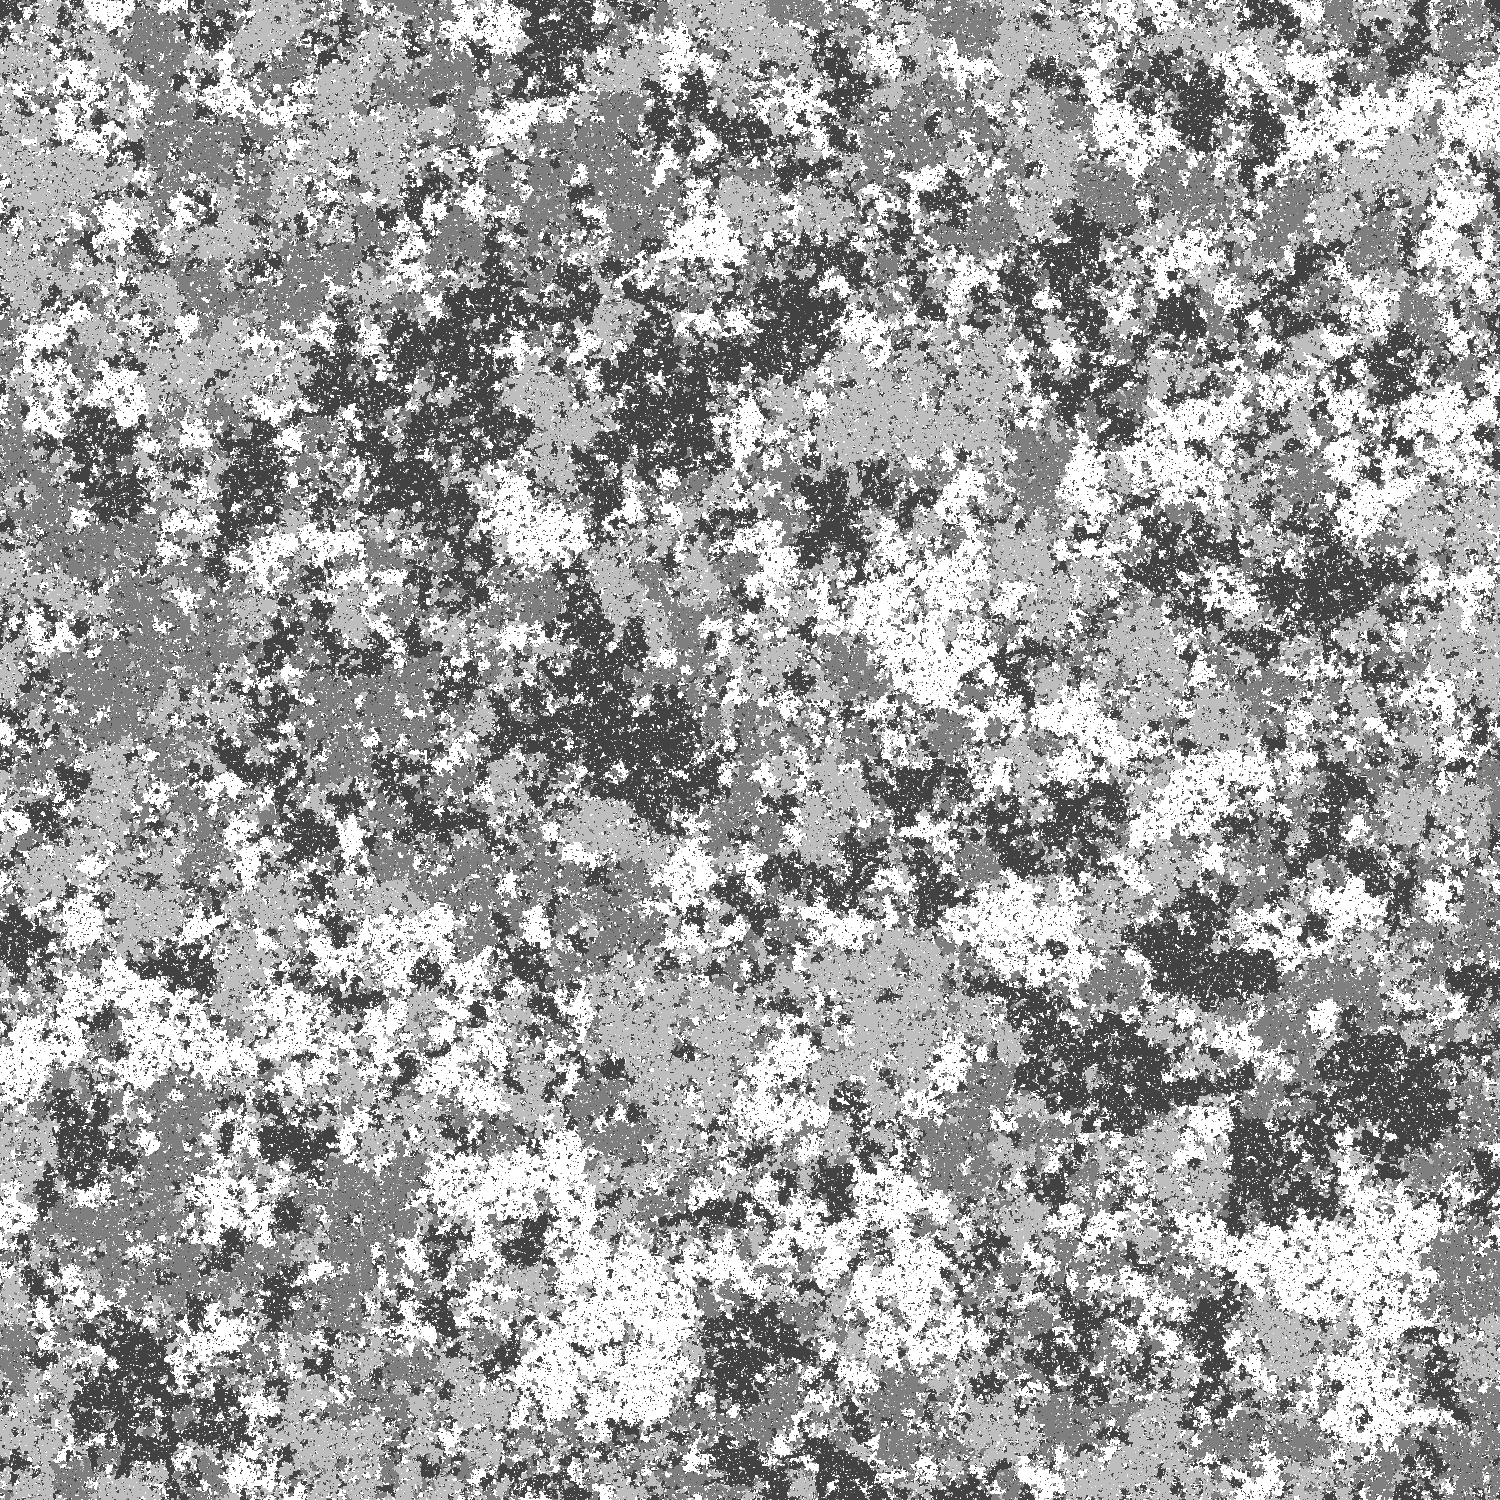
\includegraphics{../../../Images/PNG/fig1Mask_classes1.png}

}

\subcaption{\label{fig-1a}Figure 1}

\end{minipage}%
%
\begin{minipage}{0.50\linewidth}

\centering{

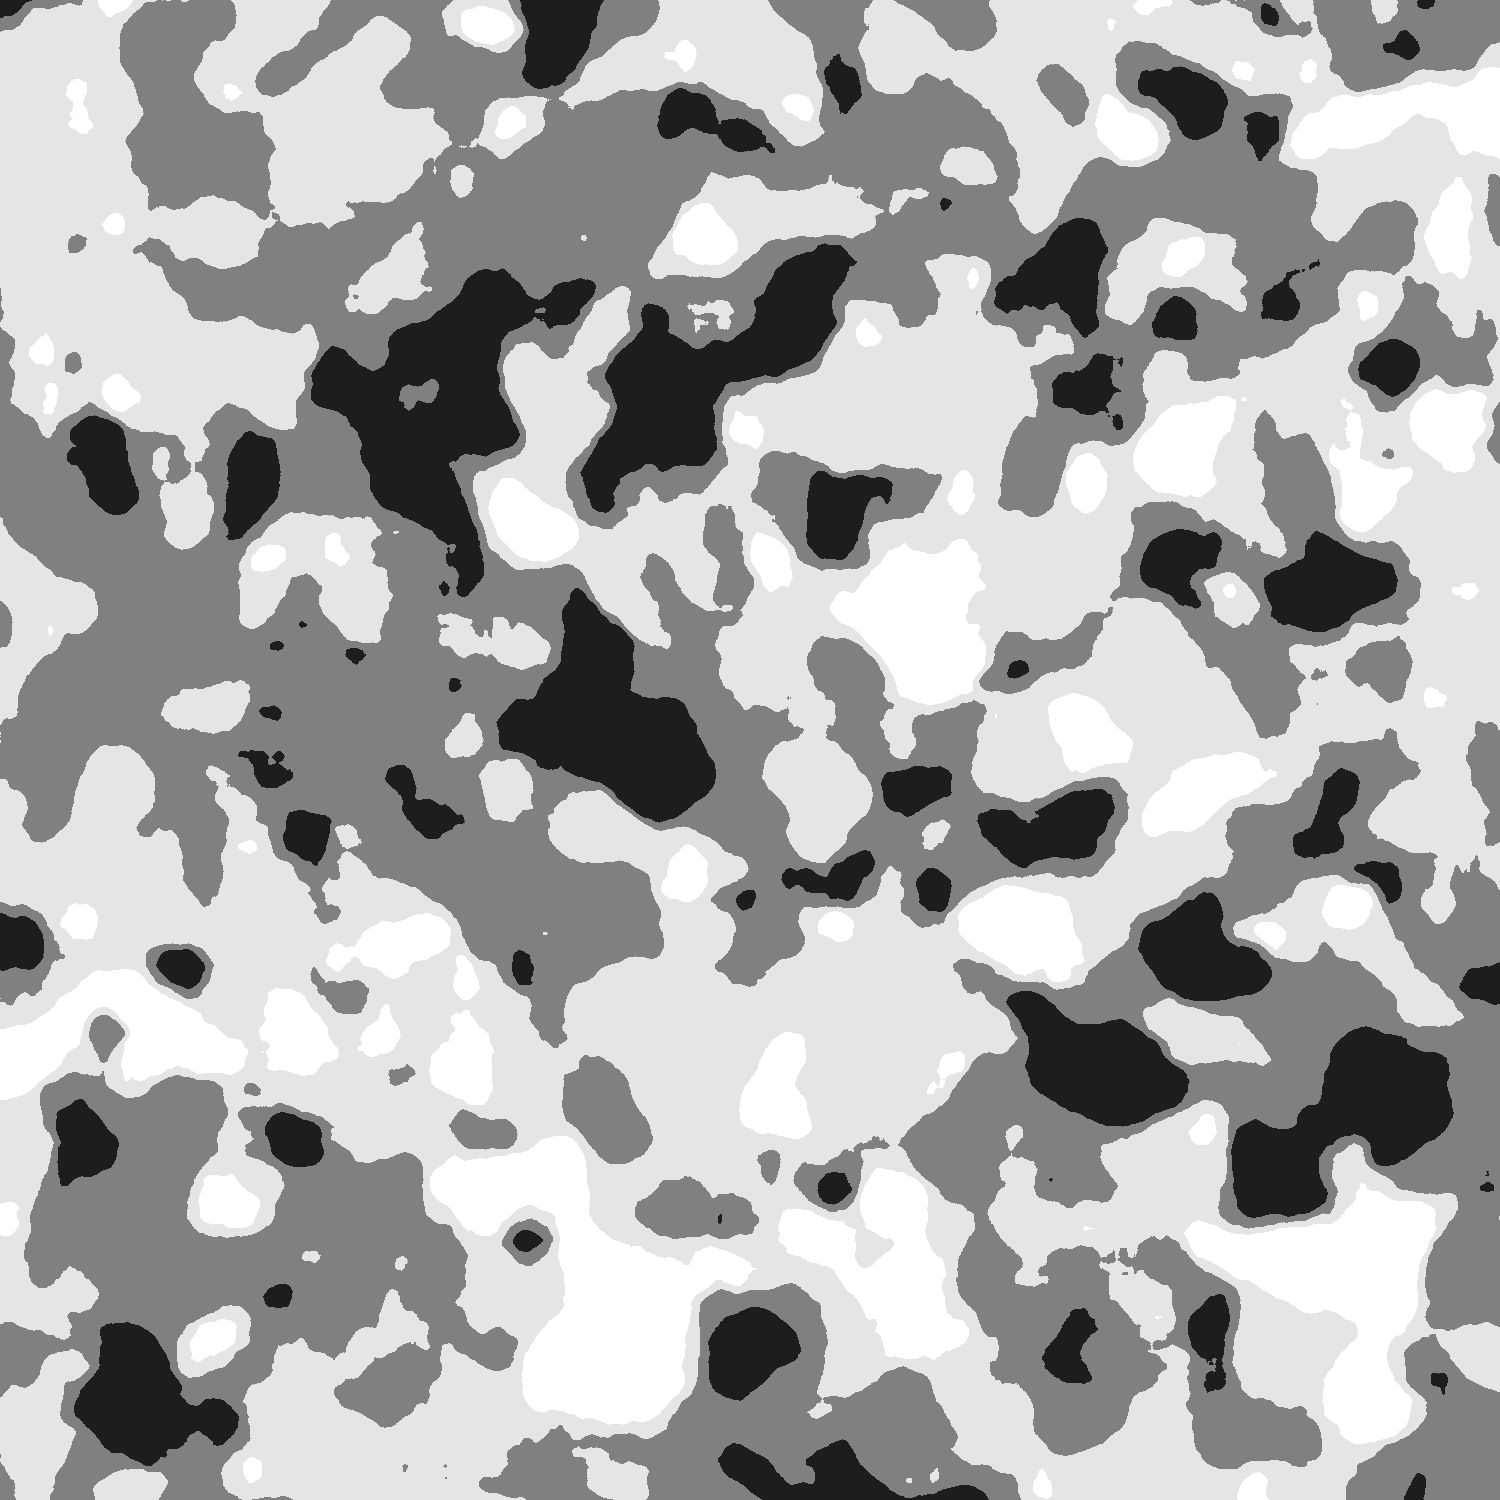
\includegraphics{../../../Images/PNG/fig1Mask_classes1_median.png}

}

\subcaption{\label{fig-1b}Figure 2}

\end{minipage}%

\end{figure}%

\subsection{Building the Dataset}\label{building-the-dataset}

The run time to get the images of the Fig.~\ref{fig-1a} and
Fig.~\ref{fig-1b} is very long. Then, to overcome this problem, we
change the processing to get the image with a dimension of
\(100\times 100\) using the MRF method with four classes. The MRF
methods got the Fig.~\ref{fig-2a}; after this, We applied the median
filter in Fig.~\ref{fig-2a}, resulting in the image shown in the
Fig.~\ref{fig-2b}.

\begin{figure}

\begin{minipage}{0.50\linewidth}

\centering{

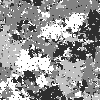
\includegraphics{../../../Images/PNG/fig1Mask_classes1_cropped.png}

}

\subcaption{\label{fig-2a}Figura 3}

\end{minipage}%
%
\begin{minipage}{0.50\linewidth}

\centering{


\includegraphics{../../../Images/PNG/fig1Mask_classes1_median_cropped.png}

}

\subcaption{\label{fig-2b}Figura 4}

\end{minipage}%

\end{figure}%

After that, we replicate a pixel of the image to a neighborhood with a
kernel defined (\(\kappa \ times \kappa\)); in this case, we use this
parameter \(\kappa = 15\) because we want to build an image with
dimensions \(1500\times 1500\). Fig.~\ref{fig-4} shows the result of
this replicate process.

\begin{figure}

\centering{


\includegraphics[width=0.3\textwidth,height=\textheight]{../../../Images/PNG/fig1Mask_classes1_cropped_repl.png}

}

\caption{\label{fig-3}}

\end{figure}%

Now, we use an arbitrary image of the Target maps of the Massachusetts
Road Dataset. We superposed this image with the image shown in
Fig.~\ref{fig-3}; its procedure generates the image shown in
Fig.~\ref{fig-4}.

\begin{figure}

\centering{

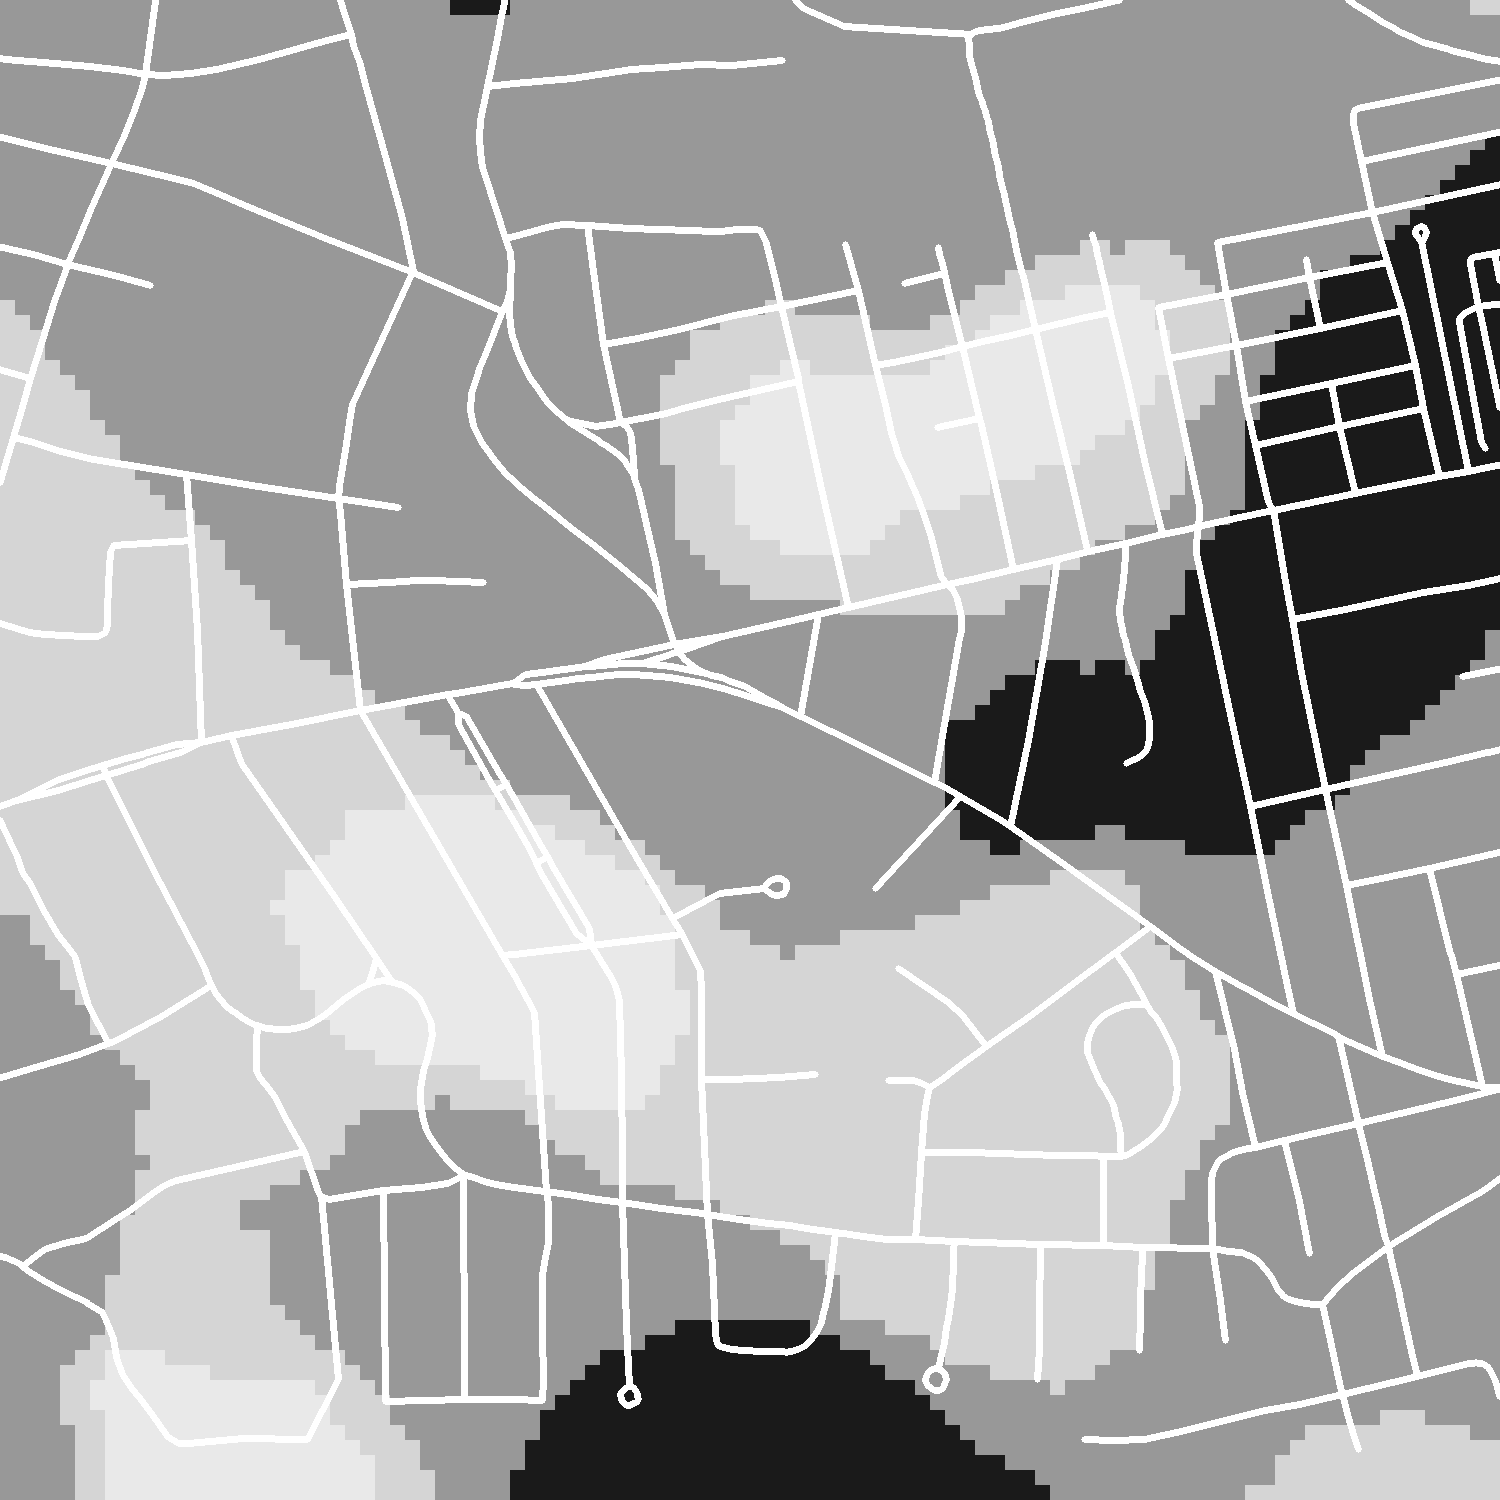
\includegraphics[width=0.3\textwidth,height=\textheight]{../../../Images/PNG/Classes1pRoads.png}

}

\caption{\label{fig-4}}

\end{figure}%

In this phase of the image simulated build, we insert gamma noise into
each of the four image classes shown in the Fig.~\ref{fig-4}.

The parameters to the gamma function to insert the noise are \(L\) and
\(\frac{L}{\text{mean}}\), where \(L=4\) and mean setting with 50, 100,
150, 200, and 500.

\subsection{Result}\label{result}

We applied the approach reported in this text to building the
Fig.~\ref{fig-5}. We can describe the image with five classes: one road
class without noise and four classes with different hypothetical noises
characterizing forest, urban, ocean, lake, agricultural cultivation,
etc.

\begin{figure}

\centering{

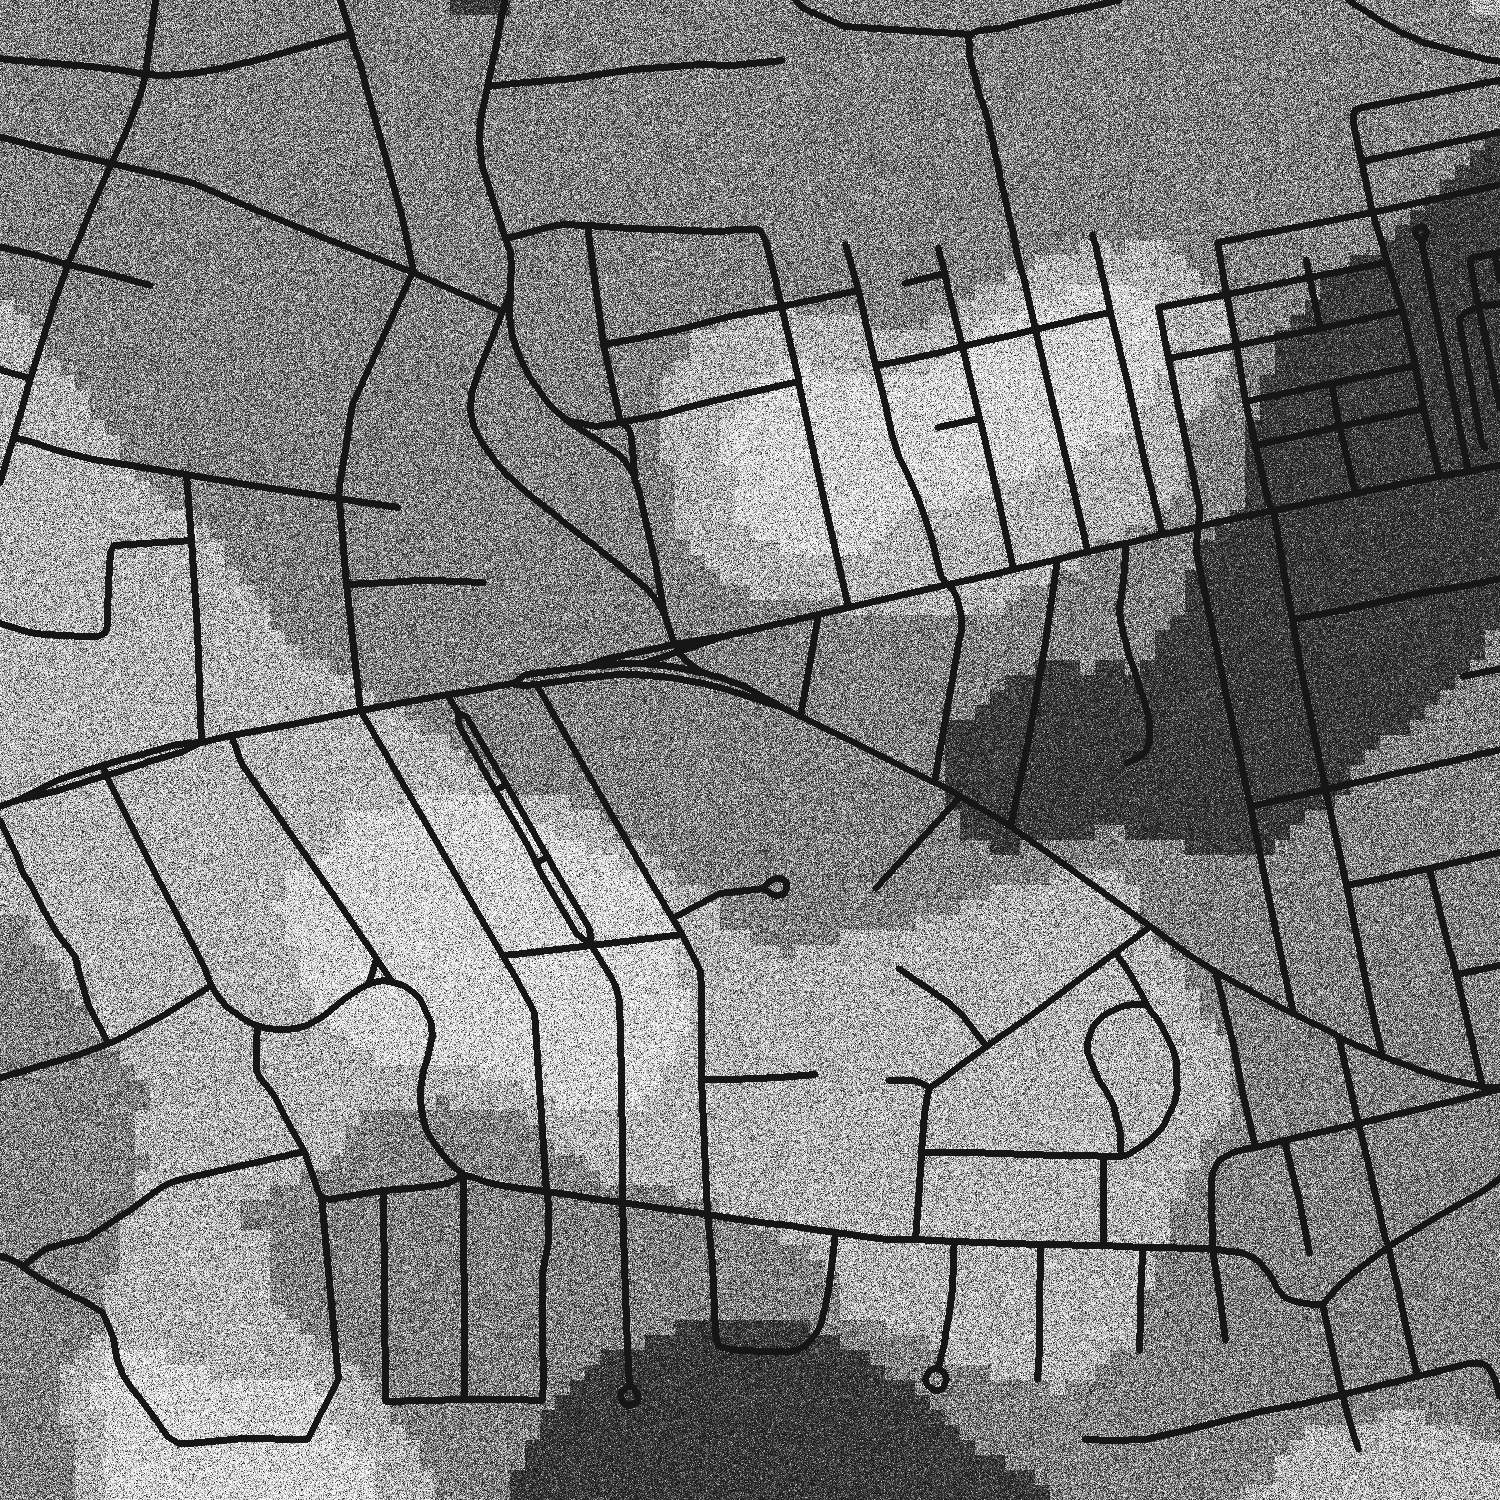
\includegraphics[width=0.3\textwidth,height=\textheight]{../../../Images/PNG/SAR1.png}

}

\caption{\label{fig-5}}

\end{figure}%

\subsection{Discussion}\label{discussion}

With the methodology described in this report, which scheme is
represented in Fig.~\ref{fig-6}, we can choose a number of the classes
in the MRF method and add gamma distribution to simulated noise in each
class defined. We now have two control parameters, the class numbers and
gamma distribution parameters (two per class). The third parameter can
be considered an image among the road maps in the Massachusetts Road
dataset, which has around one thousand road maps.

This way, we have three control parameters to build a simulated dataset
to train, validate, and test a convolutional neural network (CNN) and
apply it to the real SAR image for road detection.

Some questions.

\begin{itemize}
\item When do we use Gamma distribution or other distribution, for example, the G calligraphic distributions? Uniform or non-uniform regions? Mixed both?
\item When do we estimate the region parameters or use parameters found in the literature? The first idea can have better accuracy in the detection phase.
\end{itemize}

\begin{figure}

\centering{

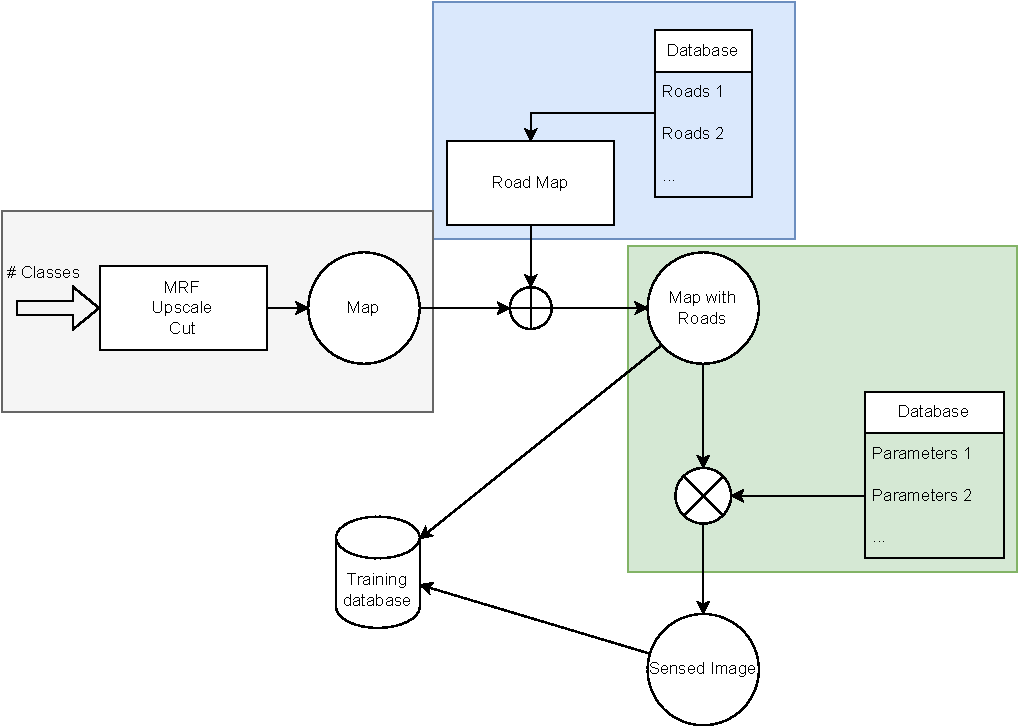
\includegraphics[width=0.51\textwidth,height=\textheight]{../../../Figures/PDF/OutlineSimulationRoads.pdf}

}

\caption{\label{fig-6}}

\end{figure}%

\section*{References}\label{references}
\addcontentsline{toc}{section}{References}

\phantomsection\label{refs}
\begin{CSLReferences}{0}{0}
\bibitem[\citeproctext]{ref-MnihThesis}
\CSLLeftMargin{{[}1{]} }%
\CSLRightInline{V. Mnih, {``Machine learning for aerial image
labeling,''} PhD thesis, University of Toronto, 2013. }

\bibitem[\citeproctext]{ref-swend_wang_1987}
\CSLLeftMargin{{[}2{]} }%
\CSLRightInline{R. H. Swendsen and J.-S. Wang, {``Nonuniversal critical
dynamics in {M}onte {C}arlo simulations,''} \emph{Phys. Rev. Lett.},
vol. 58, pp. 86--88, Jan. 1987 {[}Online{]}. Available:
\url{https://link.aps.org/doi/10.1103/PhysRevLett.58.86}}

\bibitem[\citeproctext]{ref-kroese2013handbook}
\CSLLeftMargin{{[}3{]} }%
\CSLRightInline{D. P. Kroese, T. Taimre, and Z. I. Botev, \emph{Handbook
of {M}onte {C}arlo methods}. Wiley, 2013 {[}Online{]}. Available:
\url{https://books.google.com.br/books?id=Trj9HQ7G8TUC}}

\end{CSLReferences}


% Can use something like this to put references on a page
% by themselves when using endfloat and the captionsoff option.
\ifCLASSOPTIONcaptionsoff
  \newpage
\fi

% trigger a \newpage just before the given reference
% number - used to balance the columns on the last page
% adjust value as needed - may need to be readjusted if
% the document is modified later
%\IEEEtriggeratref{8}
% The "triggered" command can be changed if desired:
%\IEEEtriggercmd{\enlargethispage{-5in}}

% Uncomment when use biblatex with style=ieee
%\renewcommand{\bibfont}{\footnotesize} % for IEEE bibfont size

\pagebreak[3]
% that's all folks
\end{document}

